\documentclass{article}
\usepackage{amsmath}
\usepackage{tikz}
\usepackage[utf8]{inputenc}
\usepackage[a4paper, top=0cm, bottom=1.8cm, left=3.3cm, right=0cm]
{geometry}
   \usepackage[absolute,overlay]{textpos}
   
   % Установка единиц измерения для textpos
   \setlength{\TPHorizModule}{1mm}
   \setlength{\TPVertModule}{1mm}
   
   \begin{document}
   
\begin{textblock*}{100mm}(0mm,0mm)
    \noindent
    \begin{minipage}{20mm}
        \includegraphics[width=\linewidth]{1.jpg} % Убедитесь, что заменили image_name.jpg на название вашего файла
    \end{minipage}%
    \begin{minipage}{90mm}
        \noindent
      The opposite sides and angles of a parallelogram are equal \textit{ and the diagonal}
        \begin{tikzpicture}[baseline={(0,-0.5ex)}]
            \draw[-] (0,0) -- (1.5,0);
            \node at (0,-0.3) {A};
            \node at (1.5,-0.3) {D};
        \end{tikzpicture}
        \textit{divides it into two equal parts.}
    \end{minipage}
\end{textblock*}
\begin{flushright}
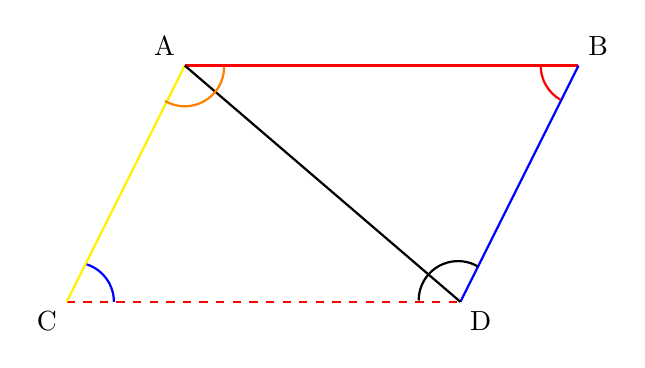
\begin{tikzpicture}

    % Draw parallelogram
    \draw[thick, dashed, red] (0,0) -- (5,0); % CD
    \draw[thick, yellow] (0,0) -- (1.5,3); % AC
    \draw[thick, red] (1.5,3) -- (6.5,3); % AB
    \draw[thick, blue] (6.5,3) -- (5,0); % BC
    
    % Diagonal
    \draw[thick, black] (1.5,3) -- (5,0); % AD
    
    % Vertex Labels
    \node at (0,0) [below left] {C};
    \node at (5,0) [below right] {D};
    \node at (1.5,3) [above left] {A};
    \node at (6.5,3) [above right] {B};

    % Draw angle arcs with colors
    \draw[thick, blue] (0.6,0.0) arc[start angle=0, end angle=72, radius=0.5];
    \draw[thick, orange] (1.25,2.55) arc[start angle=240, end angle=360, radius=0.5];
    \draw[thick, red] (6.02,3) arc[start angle=180, end angle=240, radius=0.5];
    \draw[thick, black] (5.22,0.45) arc[start angle=60, end angle=180, radius=0.5];
    
\end{tikzpicture}
\end{flushright}

\[
\left\{
\begin{array}{c}
\begin{array}{c}
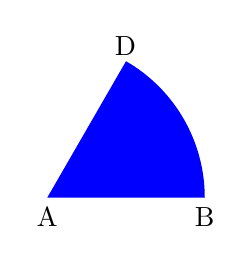
\begin{tikzpicture}
    \fill[blue]
    (0,0) coordinate (A)
    -- (2,0) coordinate (B)
    arc[start angle=0, end angle=60, radius=2]
    -- cycle;
    \node[below] at (A) {A};
    \node[below] at (B) {B};
    \node[below left] at (60:2.5) {D};
\end{tikzpicture}
\end{array}
\quad =
\begin{array}{c}
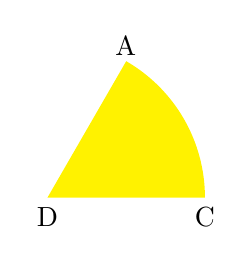
\begin{tikzpicture}
    \fill[yellow]
    (0,0) coordinate (A)
    -- (2,0) coordinate (B)
    arc[start angle=0, end angle=60, radius=2]
    -- cycle;
    \node[below] at (A) {D};
    \node[below] at (B) {C};
    \node[below left] at (60:2.5) {A};
\end{tikzpicture}
\end{array}
\\ % Переход на новую строку внутри массива
\begin{array}{c}
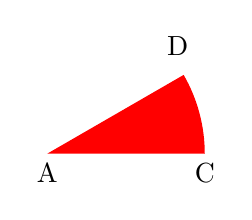
\begin{tikzpicture}
    \fill[red]
    (0,0) coordinate (A)
    -- (2,0) coordinate (B)
    arc[start angle=0, end angle=30, radius=2]
    -- cycle;
    \node[below] at (A) {A};
    \node[below] at (B) {C};
    \node[below left] at (40:2.5) {D};
\end{tikzpicture}
\end{array}
\quad =
\begin{array}{c}
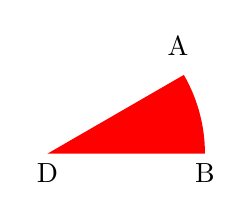
\begin{tikzpicture}
    \fill[red]
    (0,0) coordinate (A)
    -- (2,0) coordinate (B)
    arc[start angle=0, end angle=30, radius=2]
    -- cycle;
    \node[below] at (A) {D};
    \node[below] at (B) {B};
    \node[below left] at (40:2.5) {A};
\end{tikzpicture}
\end{array}
\end{array}
\right\}
\]
\[
\left\{
\begin{array}{c}
\begin{array}{c}
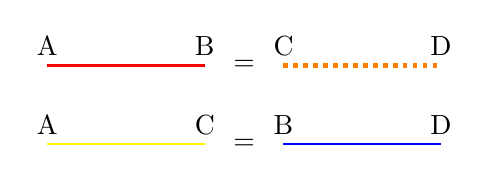
\begin{tikzpicture}
    % First row
    \draw[thick, red] (0, 0) -- (2, 0);
    \node[anchor=south] at (0, 0) {\textcolor{black}{A}};
    \node[anchor=south] at (2, 0) {\textcolor{black}{B}};
    \node at (2.5, 0) {$=$};
    \draw[ultra thick, dotted, orange] (3, 0) -- (5, 0);
    \node[anchor=south] at (3, 0) {\textcolor{black}{C}};
    \node[anchor=south] at (5, 0) {\textcolor{black}{D}};

    % Second row
    \draw[thick, yellow] (0, -1) -- (2, -1);
    \node[anchor=south] at (0, -1) {\textcolor{black}{A}};
    \node[anchor=south] at (2, -1) {\textcolor{black}{C}};
    \node at (2.5, -1) {$=$};
    \draw[thick, blue] (3, -1) -- (5, -1);
    \node[anchor=south] at (3, -1) {\textcolor{black}{B}};
    \node[anchor=south] at (5, -1) {\textcolor{black}{D}};
\end{tikzpicture}

\end{array}
\\ % Переход на новую строку внутри массива
\begin{array}{c}
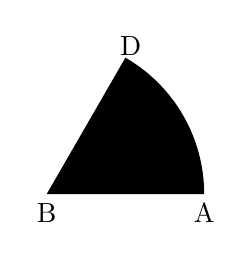
\begin{tikzpicture}
    \fill[black]
    (0,0) coordinate (A)
    -- (2,0) coordinate (B)
    arc[start angle=0, end angle=60, radius=2]
    -- cycle;
    \node[below] at (A) {B};
    \node[below] at (B) {A};
    \node[below left] at (58:2.5) {D};
\end{tikzpicture}
\end{array}
\quad =
\begin{array}{c}
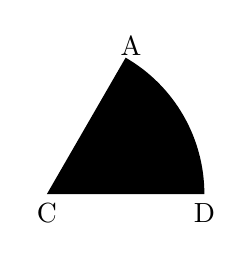
\begin{tikzpicture}
    \fill[black]
    (0,0) coordinate (A)
    -- (2,0) coordinate (B)
    arc[start angle=0, end angle=60, radius=2]
    -- cycle;
    \node[below] at (A) {C};
    \node[below] at (B) {D};
    \node[below left] at (58:2.5) {A};
\end{tikzpicture}
\end{array}
\end{array}
\right\}
\]
\centering
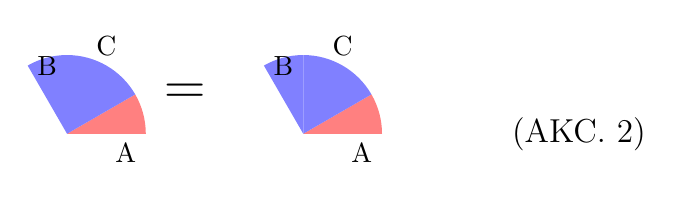
\begin{tikzpicture}
    \def\r{1}

    % Первая фигура
    \fill[red!50] (0,0) -- (0:\r) arc[start angle=0, end angle=30, radius=\r] -- cycle;
    \fill[blue!50] (0,0) -- (30:\r) arc[start angle=30, end angle=90, radius=\r] -- cycle;
    \fill[blue!50] (0,0) -- (90:\r) arc[start angle=90, end angle=120, radius=\r] -- cycle;
    \path (0,0) -- (0:\r) node[anchor=north east] {A};
    \path (0,0) -- (120:\r) node[anchor=west] {B};
    \path (0,0) -- (60:\r) node[anchor=south] {C};
    \path (0:\r) arc [start angle=0, end angle=120, radius=\r];

    % Знак равенства
    \node at (1.5,0.5) {\huge$=$};

    % Вторая фигура (скопировано)
    \begin{scope}[shift={(3,0)}]
        \fill[red!50] (0,0) -- (0:\r) arc[start angle=0, end angle=30, radius=\r] -- cycle;
        \fill[blue!50] (0,0) -- (30:\r) arc[start angle=30, end angle=90, radius=\r] -- cycle;
        \fill[blue!50] (0,0) -- (90:\r) arc[start angle=90, end angle=120, radius=\r] -- cycle;
        \path (0,0) -- (0:\r) node[anchor=north east] {A};
        \path (0,0) -- (120:\r) node[anchor=west] {B};
        \path (0,0) -- (60:\r) node[anchor=south] {C};
        \path (0:\r) arc [start angle=0, end angle=120, radius=\r];
    \end{scope}

    % Добавление текста после конструкции
    \node at (6.5,0) {\large(AKC. 2)};
    
\end{tikzpicture}

Therefore, opposite sides and angles of a parallelogram are equal. And since triangles
\begin{center}
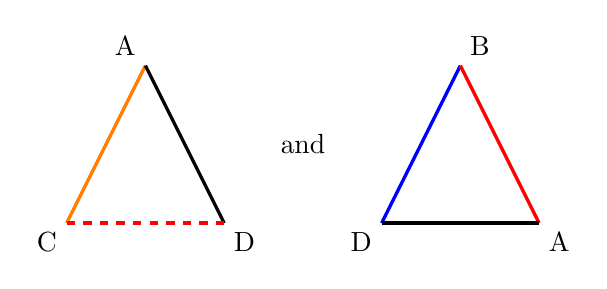
\begin{tikzpicture}[scale=1]
% Первый равносторонний треугольник
\coordinate [label=above left:A] (A1) at (0,2);
\coordinate [label=below left:C] (C) at (-1,0);
\coordinate [label=below right:D] (D1) at (1,0);

% Ребра первого треугольника
\draw[very thick, orange] (A1) -- (C);
\draw[very thick, black] (A1) -- (D1);
\draw[dashed, very thick, red] (C) -- (D1);

% Текст "and"
\node at (2,1) {and};

% Второй равносторонний треугольник
\coordinate [label=above right:B] (B) at (4,2);
\coordinate [label=below left:D] (D2) at (3,0);
\coordinate [label=below right:A] (A2) at (5,0);

% Ребра второго треугольника
\draw[very thick, blue] (B) -- (D2);
\draw[very thick, red] (B) -- (A2);
\draw[very thick, black] (D2) -- (A2);

\end{tikzpicture}
\end{center}


equal in all respects (example I.4), the diagonal divides the parallelogram into two equal parts.
 \end{document}